\documentclass[a4paper,14pt]{extreport}
\usepackage[utf8]{inputenc}
\usepackage[T2A]{fontenc}
\usepackage[russian]{babel}
\usepackage{eufrak}
% поля:
\usepackage[left=2.5cm, right=1.5cm, top=2cm, bottom=2cm]{geometry}
\linespread{1}
\usepackage{indentfirst} % отделять первую строку раздела абзацным отступом
\setlength\parindent{5ex}
\addto{\captionsrussian}{\renewcommand*{\contentsname}{Содержание}}
\usepackage[hidelinks]{hyperref} % гиперссылки в содержании
\usepackage{graphicx}
\usepackage{float}
\usepackage{amsmath}
\renewcommand*{\thesection}{\arabic{section}}

\usepackage{multirow}
\usepackage[normalem]{ulem}
\useunder{\uline}{\ul}{}

\usepackage{cmap}%позволяет копировать кириллицу из скомпилированного файла

% Глубина разделов, попадающих в содержание
\setcounter{tocdepth}{5}

\linespread{1.3} % настройка межстрочного интервала
\tolerance=1000 % настройка чувствительности вставки переносов
\hfuzz=0pt
\sloppy

\begin{document}
	\tableofcontents
	\newpage
	\section*{Введение}
	
	Целью прохождения производственной практики являлось закрепление теоретических и практических знаний, полученных при изучении дисциплин специальности и специализации, и приобретение навыков работы по избранной специальности. 
	
	Основными задачами являлись ознакомление с организацией студенческого конструкторского бюро, реализация курса лабораторных работ дисциплины “Введение в специальность”, автором которого является к.т.н. Капитонов А. А., на конструкторе Lego EV3, используя язык программирования Python.
	
	Необходимость этого курса заключается в том, что конструктор Lego NXT во-первых, снят с производства и, во-вторых, новая модель конструктора обладает большими возможностями как для обучения, так и для научный исследований. На контроллере Lego EV3 установлена полноценная операционная система Linux Debian.
	Язык программирования python был выбран так как он достаточно широко распространен в научном сообществе по причине простоты, удобства и очень широкого круга задач, решаемых при помощи стандартных библиотек.
	
	В процессе выполнения задания необходимо было закрепить теоретические знания в таких областях, как описание динамики робототехнических систем, идентификация параметров объекта управления и теория автоматического управления. 
	
	\newpage
	\section*{Основная часть}
	
	Производственную практику я проходила на кафедре СУиИ в студенческом конструкторском бюро (СКБ). СКБ является научно-исследовательским объединением студентов кафедры СУиИ, которое было создано для содействия в проведении научно-исследовательских и опытно-конструкторских работ и возможного внедрения результатов научно-технической деятельности в производство, с использованием образовательного и научного потенциала кафедры.
	
	Основными целями, которые ставит перед собой СКБ, являются: интеграция студентов в сферу научных разработок, участие в соревнованиях по робототехнике и реализация студенческих проектов на базе оборудования кафедры.
	
	В целом, нашу команду интересуют самые различные направления робототехники. Судя по выполненным за прошедший год задачам, к таковым можно отнести:
	
	На сегодняшний день в СКБ реализуются широкий круг задач самых различных направлений робототехники, к ним относятся:
	\begin{itemize}
		\item Техническое зрение роботов;
		\item Картирование и локализация роботов (SLAM) (с помощью ИК датчика-дальномера и камер с глубинным изображением);
		\item Управление манипулятором;
		\item Футбол роботов.
	\end{itemize}
	
	В будущем в СКБ планируется участие в международных соревнованиях по робототехнике (в частности RoboCup и Eurobot). 
	
	Также СКБ является мощой базой для создания различной методической литературы, в том числе учебной. Моя задача заключалась в реализации курса лабораторных работ на новом конструкторе Lego EV3, с использованием широко распространенного в научной среде языка программирования Python.
	
	Первым этапом моей работы было построение математической модели большого двигателя EV3. Для этого были измерены физические параметры, встроенного в мотор EV3, двигателя постоянного тока: масса ротора, радиус ротора, индуктивность обмотки ротора и сопротивление обмотки ротора, а также коэффициент редукции мотора. 
	
	Вторым этапом являлось получение конструктивных постоянных времени.
	
	График зависимости угла поворота от времени представлен на рисунке 1.
	На графике сплошная линия представляет результаты реальной характеристики, а пунктирная линии -- результаты моделирования.
	
	\begin{figure}[h]
		\center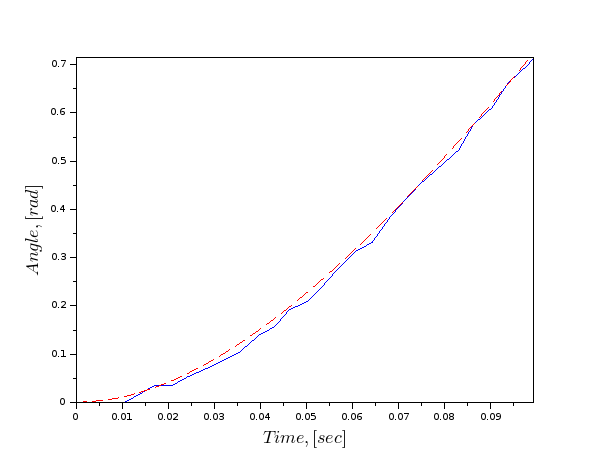
\includegraphics[width=0.8\linewidth]{angle_time.png}
		\caption{Характеристика двигателя EV3}
		\label{fig:scr1}
	\end{figure}
	
	Из полученного графика были найдены установившаяся скорость мотора $16.32$ радиан в секунду и электромеханическая постоянная времени $0.064$ сек.
	
	По полученным данным были сделаны выводы, что двигатели EV3 и NXT имею одинаковые электромеханические параметры.
	
	Третьим этапом стало написание программы управления двигателем на python. Был реализован пропорциональный регулятор и построены графики стабилизации в заданном положении. На графике сплошной линией показана реальная характеристика, а пунктирной -- результаты моделирования.
	
	\begin{figure}[H]
		\center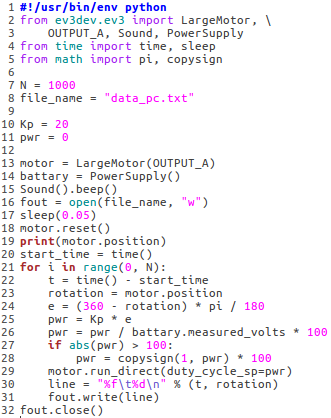
\includegraphics[width=0.5\linewidth]{listing1.png}
		\caption{Пропорциональный регулятор на python}
		\label{fig:scr1}
	\end{figure}
	\begin{figure}[H]
		\center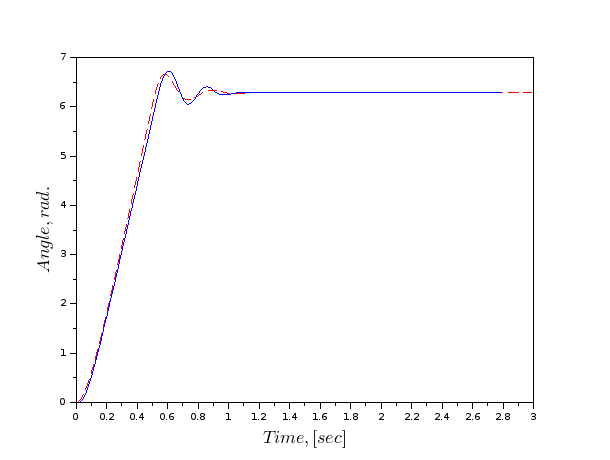
\includegraphics[width=0.7\linewidth]{angle_time2.png}
		\caption{Результаты работы пропорционального регулятора}
		\label{fig:scr1}
	\end{figure}
	
	На четвертом этапе, была построена математическая модель перевернутого маятника и расчитан регулятор.
	
	\begin{figure}[H]
		\center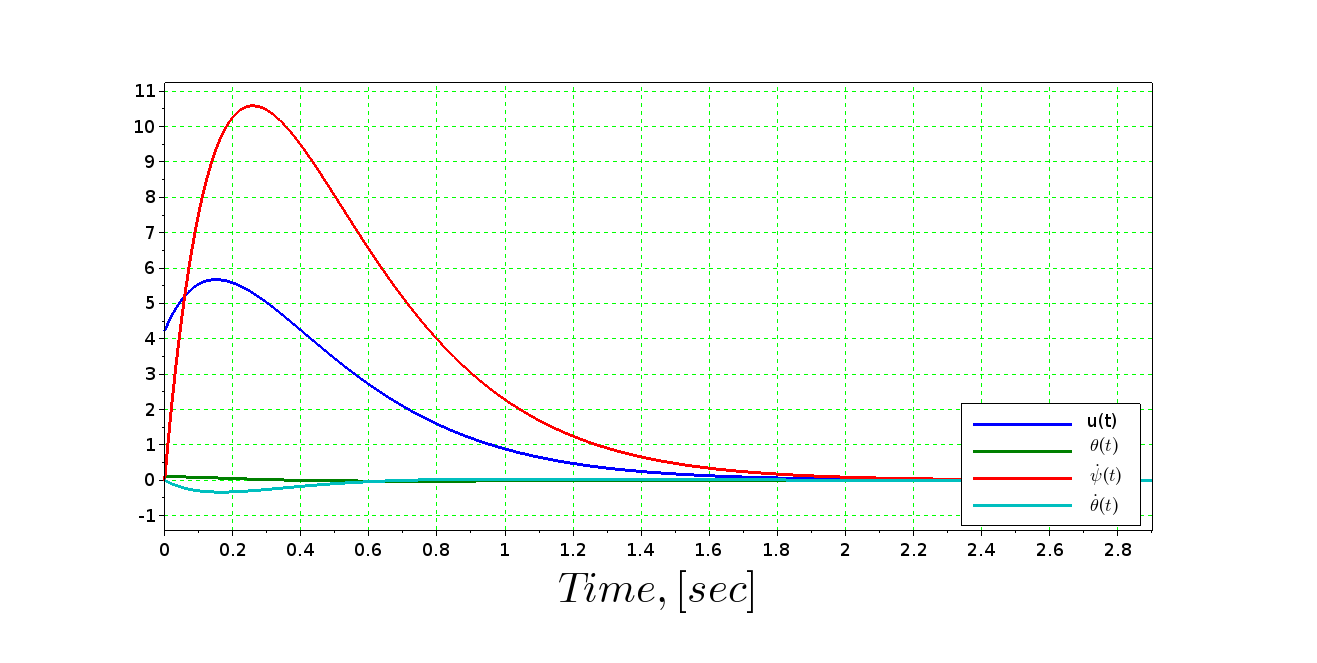
\includegraphics[width=1\linewidth]{pend4.png}
		\caption{Результаты моделирования перевернутого маятника на тележке}
		\label{fig:scr1}
	\end{figure}
	
	На пятом этапе была собрана реальная модель, написана программа управления на python и настроена.
	
	Из особенностей, следует заметить, что регулятор был рассчитан в результате решения матричного уравнения Сильвестра.
	
	Также, в существующих библиотеках python для Lego EV3 не была реализована возможность работы с датчиком угла поворота Lego HTAngleSensor, что было исправлено путем ее реализации.
	
	
	\begin{figure}[H]
		\center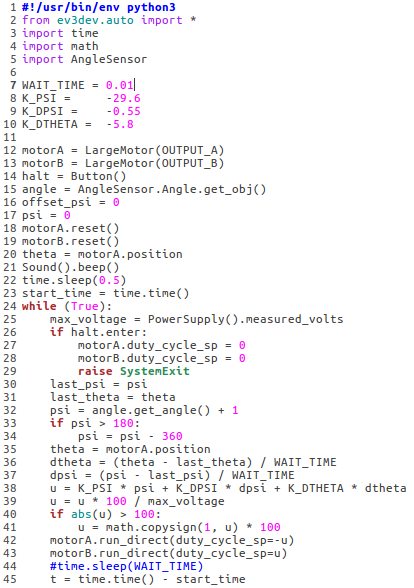
\includegraphics[width=0.7\linewidth]{listing2.png}
		\caption{Программа стабилизации перевернутого маятника на тележке для Lego EV3}
		\label{fig:scr1}
	\end{figure}
	
	\newpage
	\section*{Заключение}
	
	В результате проделанной работы, был полностью повторен курс лабораторных работ для более нового набора Lego EV3. Было отмечено, что разработка программы на python под привычную операционную может быть не только полезным, а также может приносить массу удовольствия от самого процесса. На контроллере был настроен репозиторий и система онлайн отладки программы. Подключение контроллера к компьютеру производилось по беспроводной сети WiFi, что существенно упрощает отладку, снятие показаний работы робота, просмотр логов и статистики работы программы.
	
	В последствии стоит, переработать написанные программы в соответствии сегодняшними тенденциями развития языков программирования на python3 c применением парадигмы программирования ООП.
	
	Также необходимо будет настроить операционную систему ROS на контроллере LegoEV3, произвести тесты производительности, в случае позитивных показаний которых, возможно будет реализовать техническое зрения для этого контроллера.
	
	\newpage
	\section*{Список использованных источников}
	
\end{document}

